% Created 2018-07-21 Sat 19:25
\documentclass[bigger]{beamer}
\usepackage[utf8]{inputenc}
\usepackage[T1]{fontenc}
\usepackage{fixltx2e}
\usepackage{graphicx}
\usepackage{longtable}
\usepackage{float}
\usepackage{wrapfig}
\usepackage{rotating}
\usepackage[normalem]{ulem}
\usepackage{amsmath}
\usepackage{textcomp}
\usepackage{marvosym}
\usepackage{wasysym}
\usepackage{amssymb}
\usepackage{hyperref}
\tolerance=1000
\usepackage{minted}
\DeclareMathOperator*{\argmin}{arg\,min}
\usepackage{subcaption}
\usepackage{graphicx}
\usetheme{Montpellier}
\author{Timothy Schwieg}
\date{\today}
\title{Valuations of Items in Counter-Strike: Global Offensive}
\hypersetup{
  pdfkeywords={},
  pdfsubject={},
  pdfcreator={Emacs 25.3.1 (Org mode 8.2.10)}}
\begin{document}

\maketitle

\section{Anyone Want a Pool Table?}
\label{sec-1}

\begin{frame}[label=sec-1-1]{The Problem}
\begin{itemize}
\item People are randomly distributed items in the game.
\item They have private valuations for each item that are not known to the
designers
\item A market is created in order to ensure an efficient outcome.
\item Takes the form of a double auction - converging to competitive equilibrium
\end{itemize}
\end{frame}

\begin{frame}[label=sec-1-2]{Matching}
\begin{itemize}
\item One context to think of the problem as one of matching individuals
in order to maximize the total surplus.
\item We know from Micro2 that this is equivalent to thinking about a
decentralized market.
\item The Objective function is valuation of the buyers and the sellers
\end{itemize}
\end{frame}

\begin{frame}[label=sec-1-3]{Who Gets What}
\begin{itemize}
\item Both buyers and sellers have the same distribution of valuations
\item However, the masses of the buyers and sellers are not equal.
\item Only some percentage are endowed with the item
\item Market is efficient - highest valuations end up with the item.
\end{itemize}
\end{frame}

\begin{frame}[label=sec-1-4]{The Planner's Problem}
\begin{align*}
\max_{\alpha_{i,j}} & \sum_{i=1}^I \sum_{j=1}^J \left ( V_i - V_j ) \alpha_{i,j} \\
\text{subject to: } & \forall j, 1 \leq j \leq J \quad \sum_{i=1}^I \alpha_{i,j} \leq 1 \\
& \forall i, 1 \leq i \leq I \quad \sum_{j=1}^J \alpha_{i,j} \leq 1\\
\end{align*}
\end{frame}

\begin{frame}[label=sec-1-5]{Planner's Problem (cont)}
\begin{itemize}
\item The solution to this is not unique.
\item The difference in valuations is both sub and super-modular. This
implies that both PAM and NAM are supported, and all permutations
between the sellers and buyers selected are supported.
\item This means we know who is matched but not with whom.
\end{itemize}
\end{frame}

\begin{frame}[label=sec-1-6]{The dual}
\begin{align*}
\min_{x,j} & \sum_{i=1}^I x_i + \sum_{j=1}^J y_j \\
\text{subject to: } & \forall i,j; \quad 1 \leq j \leq J, \quad 1 \le i \leq I\\
& x_i + y_j \geq V_i - V_j \\ 
\end{align*}

\begin{itemize}
\item This has a unique solution - for each buyer and seller it gives the
shadow price: the surplus that each commands.
\item Because the function is modular, the valuation plus the surplus for
all sellers is equal - this is the price the market supports.
\end{itemize}
\end{frame}

\begin{frame}[label=sec-1-7]{What it looks like}
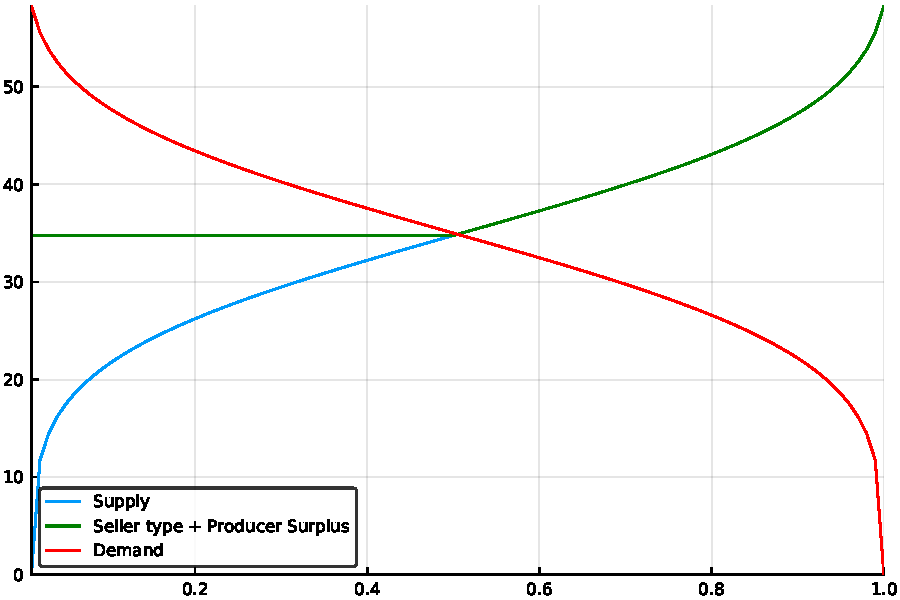
\includegraphics[width=.9\linewidth]{../Scripts/evenStevens.pdf}
\end{frame}

\begin{frame}[label=sec-1-8]{Unequal Buyers and Sellers}
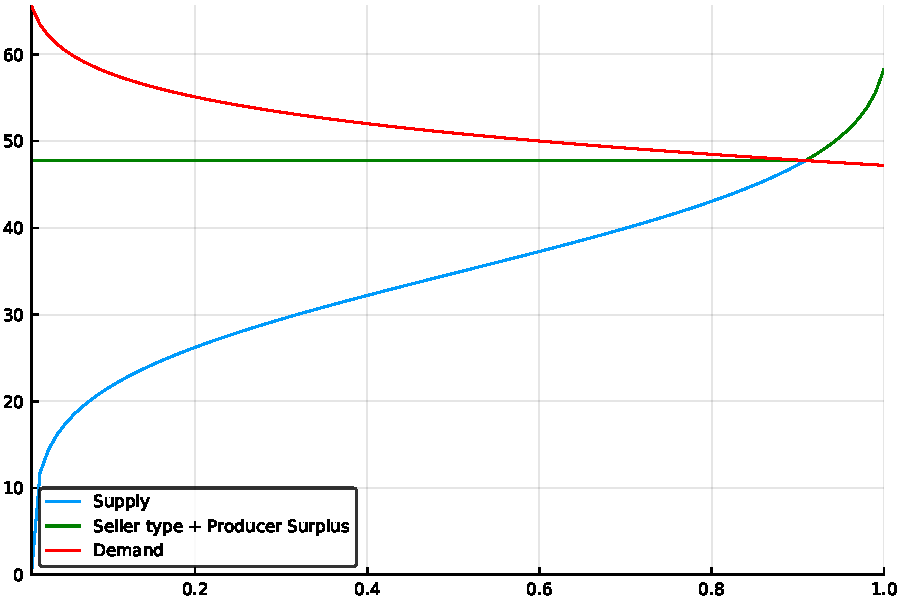
\includegraphics[width=.9\linewidth]{../Scripts/oneTenth.pdf}
\end{frame}

\begin{frame}[label=sec-1-9]{Equilibrium}
\begin{itemize}
\item Let the proportion of the population that received the item be
denoted $\xi$.
\item For normally distributed valuations, the price is defined by:
\end{itemize}

\begin{align*}
\Phi \left ( \frac{ p^* - \mu }{\sigma} \right ) &= \frac{1-\xi}{\xi} \left [ 1 - \Phi \left
( \frac{ p^* - \mu }{\sigma} \right ) \right ]\\
p^* &= \mu + \sigma \Phi^{-1} ( 1- \xi )\\
\end{align*}
\end{frame}


\begin{frame}[label=sec-1-10]{Known $\xi$}
\begin{itemize}
\item If we knew $\xi$, this model could be estimated via linear regression
\item Can handle even if there is measurement error in calculating $\xi$.
\item However, even if we know the quantity of sales, and the number of
people playing, no idea of people engaging in the market.
\item Need to use the price to endogenize $\xi$.
\end{itemize}
\end{frame}

\begin{frame}[label=sec-1-11]{Dynamic Approach}
\begin{itemize}
\item Let this process repeat over many time intervals.
\item Assume no entry into the market.
\item Since this market is efficient, the top portion of the buyers always
purchases the item, and the price slowly falls
\item This can only support a decreasing price.
\end{itemize}
\end{frame}

\begin{frame}[label=sec-1-12]{A Simulation}
\begin{itemize}
\item $\mu = 0, \sigma = 1, \xi = .05, N = 1000, T = 40$
\end{itemize}
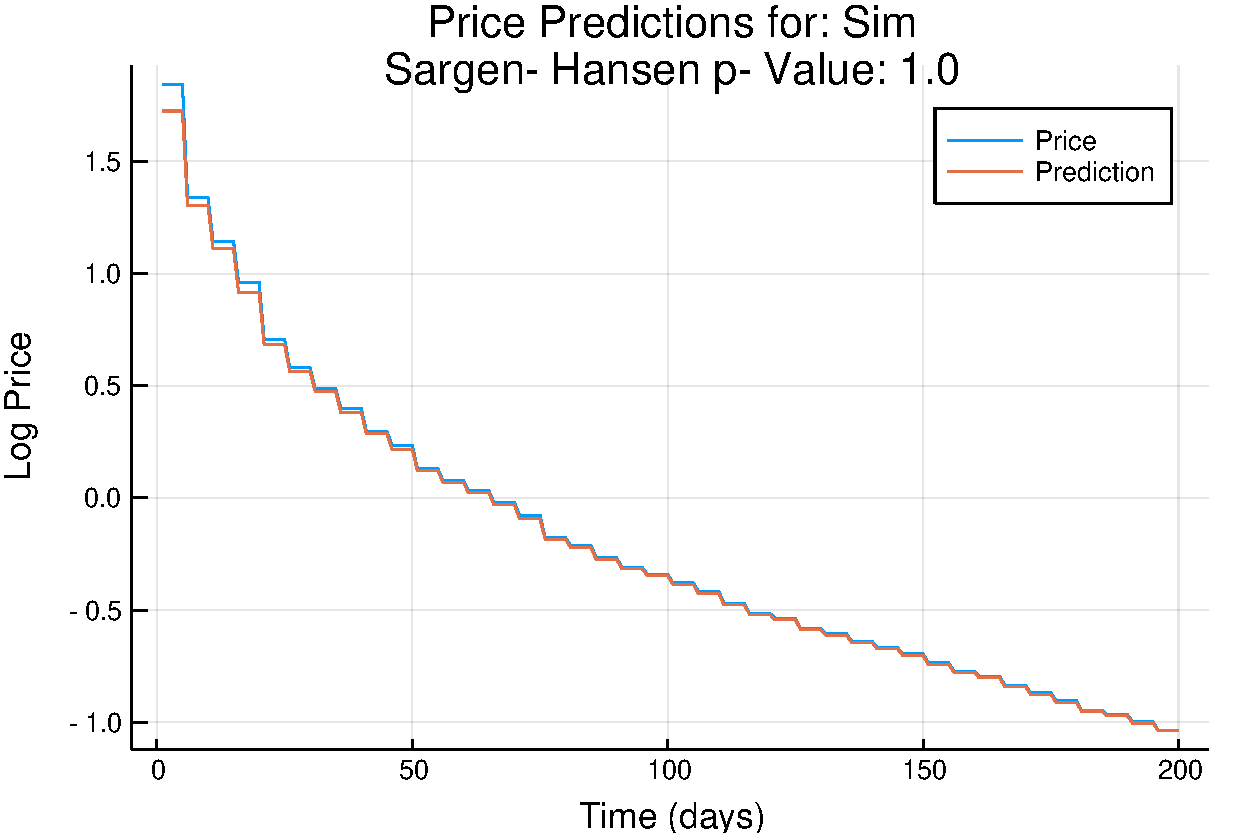
\includegraphics[width=.9\linewidth]{../Plots/Sim.pdf}
\end{frame}

\begin{frame}[label=sec-1-13]{Specification}
\begin{align*}
\mathbb{E}[ q_s ] &= N \prod_{t=0}^{T-1} (1-\xi_t ) \xi_T \frac{\Phi \left ( \frac{ \log ( p_T^* ) - \mu }{\sigma} \right )}{ \prod_{t=0}^{T-1} ( 1 - \xi_t ) }\\
\mathbb{E}[ q_d ] &= N \prod_{t=0}^{T} ( 1- \xi_t ) \left [ 1 - \frac{ \Phi \left ( \frac{
\log ( p_T^* ) - \mu }{ \sigma } \right ) }{ \prod_{t=0}^{T-1} (1 - \xi_t ) } \right ]\\
\log ( p_T^* ) &= \mu + \sigma \Phi^{-1} \left [ \prod_{t=0}^T ( 1 - \xi_t ) \right ]\\
q_T^* &= N \prod_{t=0}^T ( 1 - \xi_t ) \xi_T \\
\end{align*}
\end{frame}



\begin{frame}[label=sec-1-14]{Problems with Data}
\begin{itemize}
\item This model cannot support the prices increasing.
\item One possibility is to add white noise, which increases the variance
on all observations, and can explain some jumps in prices.
\item This cannot explain trends in prices that are observed in some items.
\item Worse yet, it predicts price to eventually fall to zero, which is
not represented by some of the cases
\end{itemize}
\end{frame}

\begin{frame}[label=sec-1-15]{Failure in Prediction}
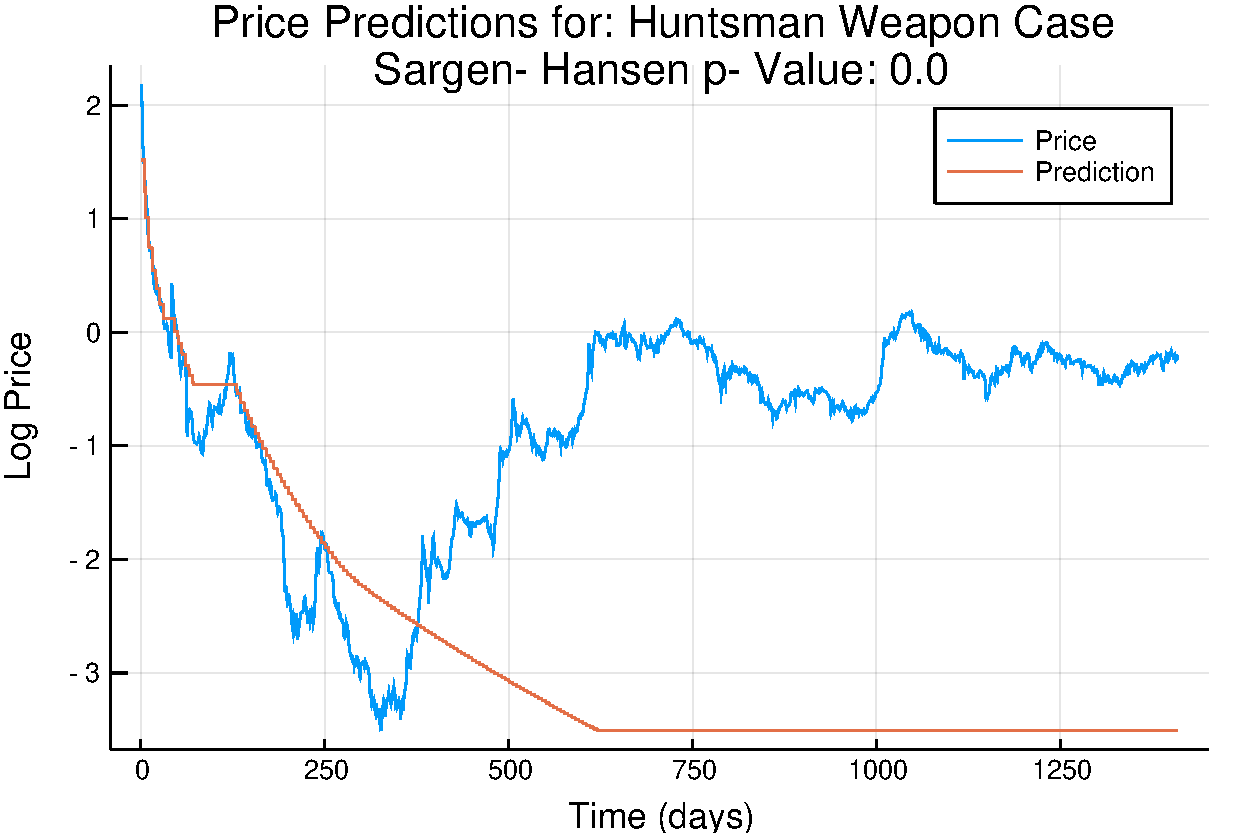
\includegraphics[width=.9\linewidth]{../Plots/Cases/Cases/HuntsmanWeaponCase.pdf}
\end{frame}

\begin{frame}[label=sec-1-16]{What can we predict?}
\begin{itemize}
\item We are predicting the price to eventually drop to zero, but we do
not have an equilibrium specification. So for data where the price
is driven on a downward trend, we can estimate the data.
\item We choose to group together data in periods of 5 days. Assume model
is in equilibrium in each of those days. This generates moments for
estimation
\end{itemize}
\end{frame}

\begin{frame}[label=sec-1-17]{Generalized Method of Moments}
\begin{itemize}
\item Function g(Y$_{\text{t}}$ ,$\mu$,$\sigma$,$\xi$) which gives the moment condition for
each time period
\end{itemize}
\begin{equation*}
\mathbb{E}[ g( Y_t, \mu, \sigma, \xi ) ] = 0
\end{equation*}
\begin{itemize}
\item Sample Analog: $\hat{m} ( \mu, \sigma, \xi ) = \frac{ 1 }{ M } \sum_{m=1}^M g( Y_m,
  \mu, \sigma, \xi )$
\end{itemize}

\begin{equation*}
\hat{\theta} = \argmin_{\theta} \hat{m}( \theta )' W \hat{m}( \theta )
\end{equation*}
\end{frame}

\begin{frame}[label=sec-1-18]{Generalized Method of Moments}
\begin{itemize}
\item What is this W matrix? How do we get it?
\item Using Iterated GMM Estimator
\end{itemize}

\begin{align*}
\hat{W_i} &= \left [ \frac{1}{M} \sum_{m=1}^M g(Y_m, \hat{\theta_{i-1}} ) g( Y_m, \hat{\theta_{i-1}} )' \right ]^{-1} \\
\hat{\theta_i} &= \argmin_{\theta} \hat{m}( \theta_i )' \hat{W_i} \hat{m}( \theta_i ) \\
\end{align*}
\end{frame}

\begin{frame}[label=sec-1-19]{Complication?}
\begin{itemize}
\item Forming W this way involves inverting a matrix that may not be of
full rank.
\item Add some positive number times the identity matrix in order to
obtain full rank as well as positive definiteness.
\item One advantage of the Iterated Method is that the W matrix formed is
invariant to the scale of the data, which is especially important
for this data
\end{itemize}
\end{frame}

\begin{frame}[label=sec-1-20]{Monte Carlo}
\begin{itemize}
\item However, we are still estimating a dynamic system, and that is
notoriously difficult.
\item This is especially the case in our model since early estimated
values of $\xi$ have a large impact on the later values.
\item These tests were not conducted near the magnitude of the data
collected, as solving LPs of that size ( 10$^{\text{13}}$ ) is not feasible
\item These simulations may overstate the role of random noise.
\end{itemize}
\end{frame}

\begin{frame}[label=sec-1-21]{Monte Carlo}
\begin{itemize}
\item I ran 1000 simulations of this model, all with N = 1000, $\mu$ = 0, $\sigma$ =
1, $\xi$ = 0.05, T = 50.
\item Tested: Sargan Hansen Test, LR Test for $\xi$ constant, LR Test for $\mu$
  =0, $\sigma$ = 1, $\xi$ = 0.05
\item Rejected with $\alpha$ = 0.05
\end{itemize}

\begin{center}
\begin{tabular}{lrrr}
 & Sargan Hansen & $\xi$ constant & Simulation Primitives\\
Reject \% & 3.7 & 44.0 & 100.0\\
\end{tabular}
\end{center}
\end{frame}


\begin{frame}[label=sec-1-22]{Some Predictions}
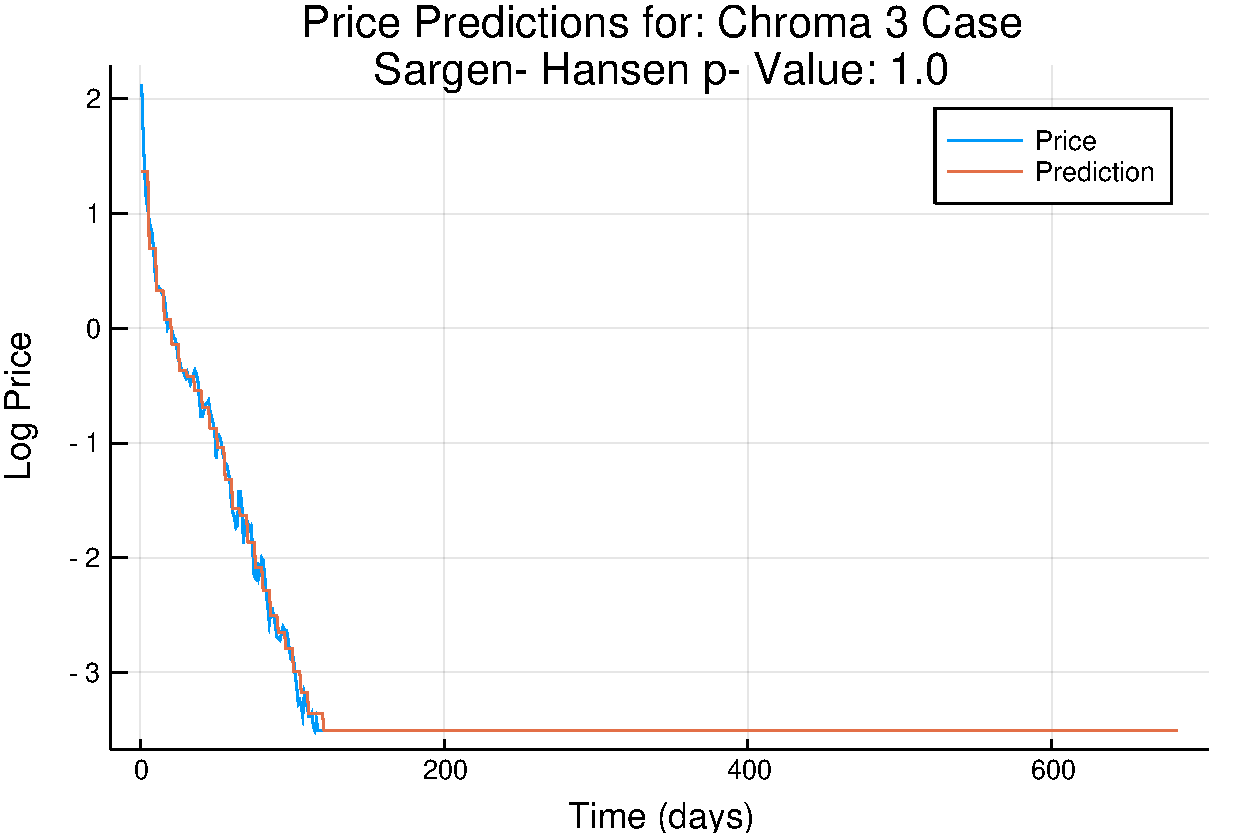
\includegraphics[width=.9\linewidth]{../Plots/Cases/Cases/Chroma3Case.pdf}
\end{frame}

\begin{frame}[label=sec-1-23]{Some Predictions}
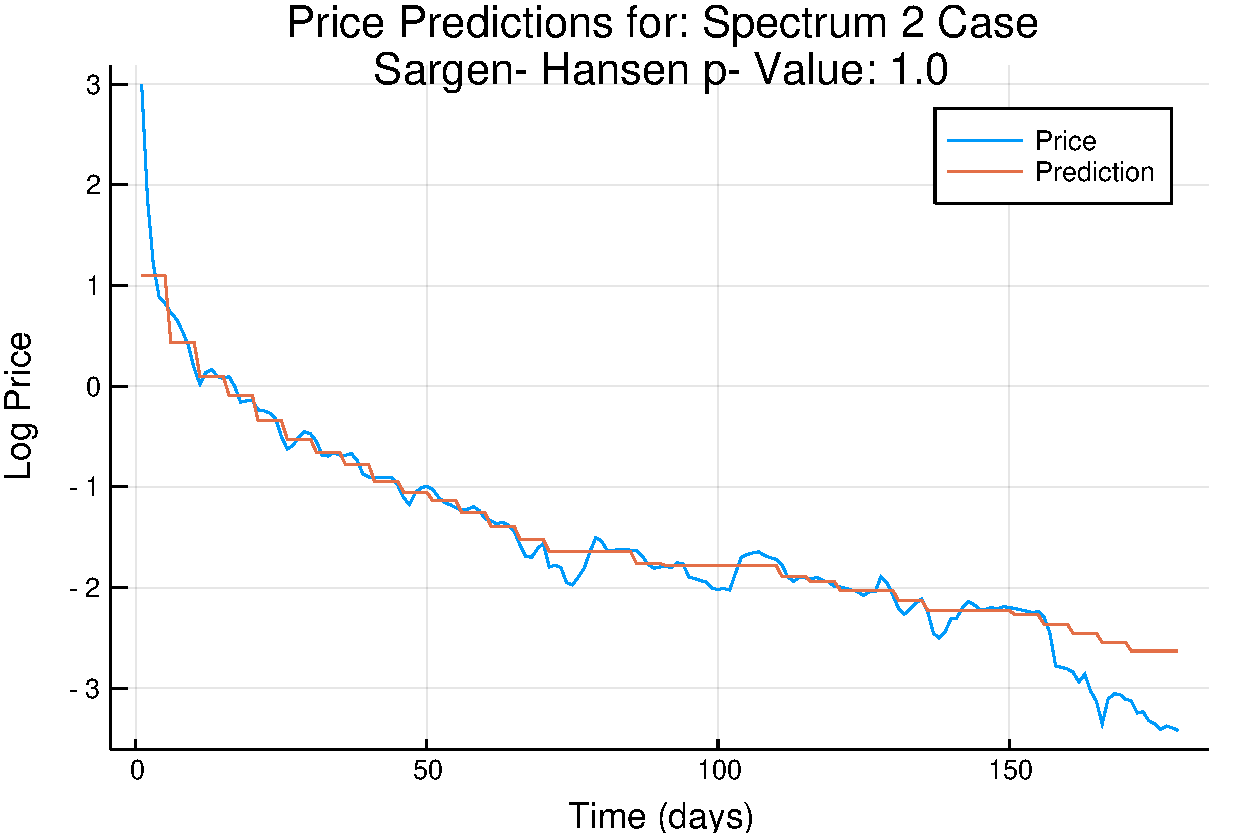
\includegraphics[width=.9\linewidth]{../Plots/Cases/Cases/Spectrum2Case.pdf}
\end{frame}

\begin{frame}[label=sec-1-24]{Some Predictions}
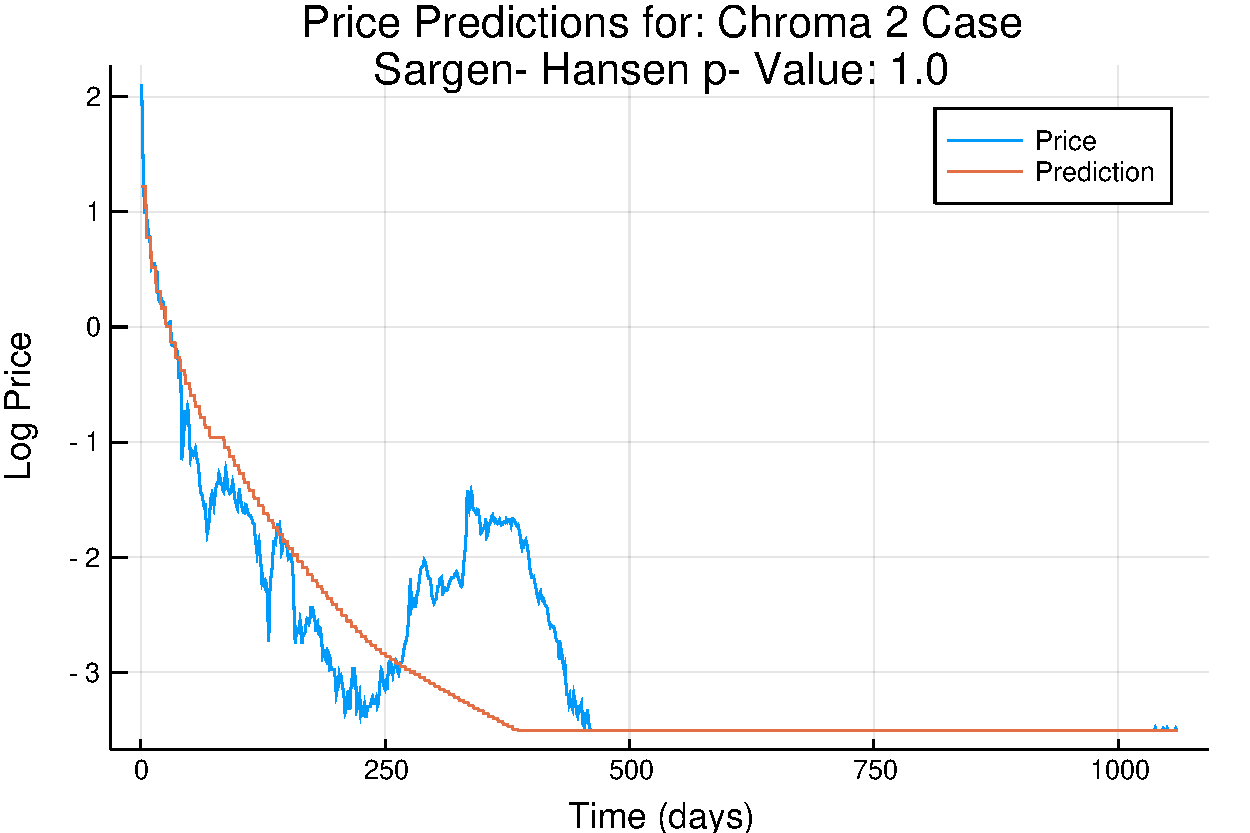
\includegraphics[width=.9\linewidth]{../Plots/Cases/Cases/Chroma2Case.pdf}
\end{frame}

\begin{frame}[label=sec-1-25]{Some Predictions}
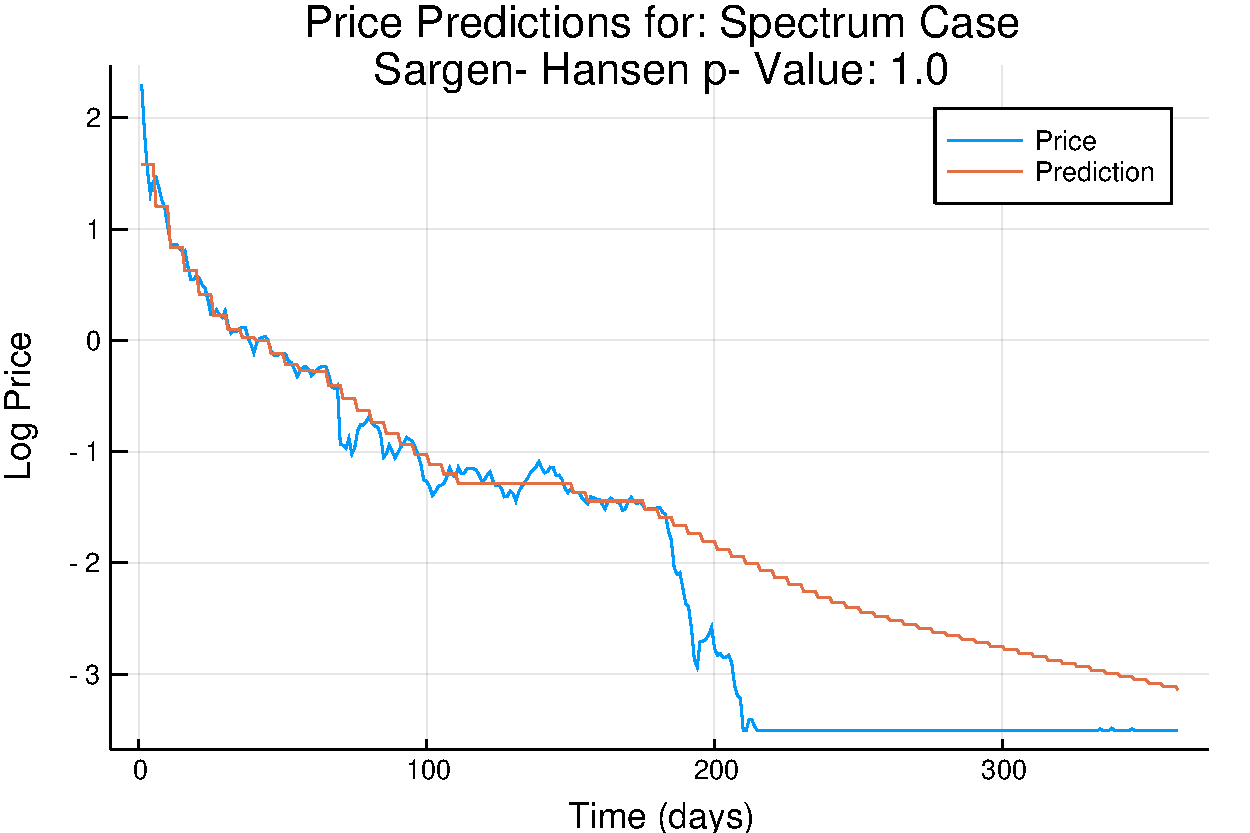
\includegraphics[width=.9\linewidth]{../Plots/Cases/Cases/SpectrumCase.pdf}
\end{frame}


\begin{frame}[label=sec-1-26]{Market Entry}
\begin{itemize}
\item For the price to be able to increase, there must be new people
entering the market.
\item Let $\lambda$$_{\text{t}}$ denote the percent of new entrants into the market.
\item Since each new entrant has the original valuations, we must consider
all owners of the item, even past owners.
\item This leads to both buyers and sellers having a mixing distribution
of valuations
\end{itemize}
\end{frame}

\begin{frame}[label=sec-1-27]{Masses of Buyers and Sellers}
\begin{align*}
M_B(T) &= N (1-\xi_T ) \prod_{t=0}^{T-1} ( 1 - \xi_t + \lambda_t ) \\
M_S(T) &= N \sum_{i = 0}^T \xi_i \prod_{t=0}^{i-1} ( 1- \xi_t + \lambda_t )\\
M_B(T) &= N B_T ( p_T )\\
M_S(T) &= N \left ( 1 - B_T(p_T) + \sum_{t=1}^{T-1}  R_{t}(\lambda,p) \right )\\
R_i(\lambda,p) &= \lambda_i \left [ B_{i-1}(p_{i-1} ) + R_{i-1}(\lambda, p) \right ]\\
R_0 (\lambda,p) &= \lambda_0 \\
\end{align*}
\end{frame}

\begin{frame}[label=sec-1-28]{Valuations of Buyers and Sellers}
\begin{align*}
B_T (p) &= \frac{ B_{T-1 }(p_{T-1}) }{ B_{T-1 }(p_{T-1}) + \lambda_1 } \min \left \{ 1, \frac{ B_{T-1} ( p ) }{B_{T-1 }(p_{T-1 })} \right \}\\
 & \quad + \frac{ \lambda_1 }{ B_{T-1 }(p_{T-1}) + \lambda_1 } B_0 (p) \\
S_T (p) &= \frac{ M_S(T-1) }{ M_S(T) } \max \left \{ 0, \frac{ B_{T-1}(p) - B_{T-1}( p_{T-1} ) }{ 1 - B_{T-1} ( p_{T-1} ) } \right \}\\
 & \quad + \frac{ M_S(T) - M_S(T-1)_{} }{M_S(T)} B_T (p)\\
\end{align*}


\begin{itemize}
\item $B_t(p)$ and $S_t(p)$ are strictly increasing functions of p, so the
intersection between $q_d, q_s$ is uniquely defined.
\end{itemize}
\end{frame}
\begin{frame}[label=sec-1-29]{Problems}
\begin{itemize}
\item There are some serious identification problems with this
\end{itemize}
model
\begin{itemize}
\item 2T Moments, but 2T+2 Primitives in the model.
\item Assuming $\xi$ constant over the lifetime is one possible identification
strategy.
\item However, a bigger problem with the estimation presents itself.
\end{itemize}
\end{frame}

\begin{frame}[label=sec-1-30]{Behavior Over Time}
\begin{figure}[htb]
\centering
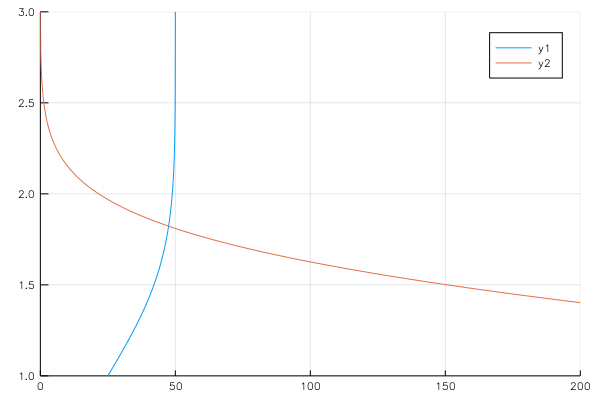
\includegraphics[width=.9\linewidth]{../Plots/gif/000001.png}
\caption{Time 1}
\end{figure}
\end{frame}


\begin{frame}[label=sec-1-31]{Behavior Over Time}
\begin{figure}[htb]
\centering
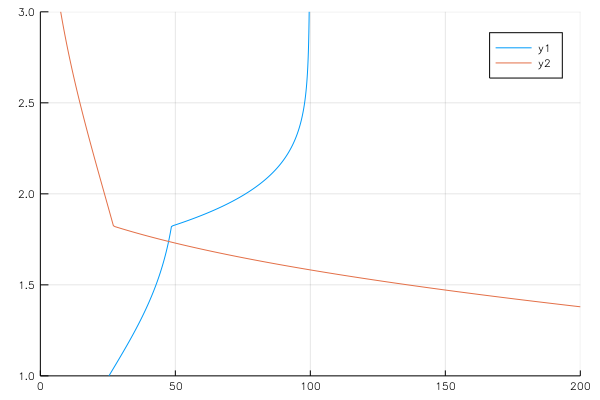
\includegraphics[width=.9\linewidth]{../Plots/gif/000002.png}
\caption{Time 2}
\end{figure}
\end{frame}


\begin{frame}[label=sec-1-32]{Behavior Over Time}
\begin{figure}[htb]
\centering
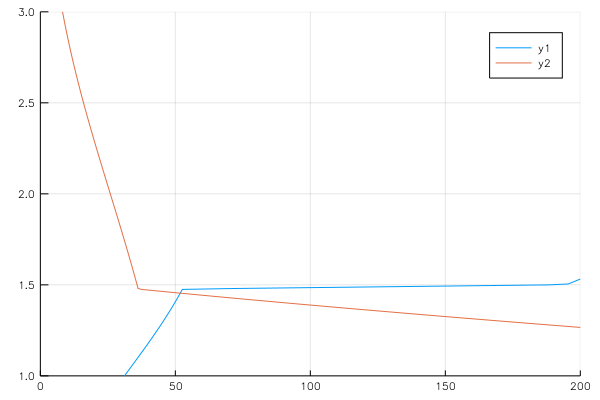
\includegraphics[width=.9\linewidth]{../Plots/gif/000010.png}
\caption{Time 10}
\end{figure}
\end{frame}


\begin{frame}[label=sec-1-33]{Behavior Over Time}
\begin{figure}[htb]
\centering
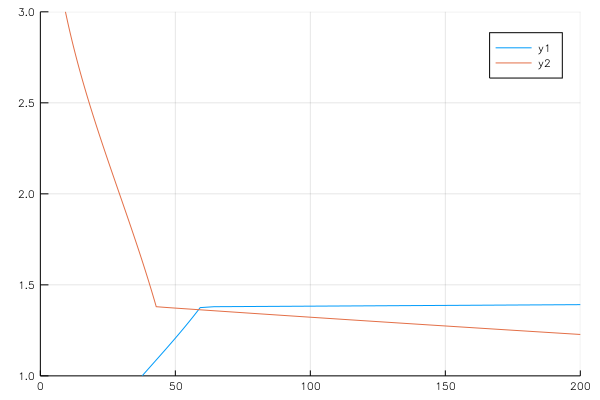
\includegraphics[width=.9\linewidth]{../Plots/gif/000015.png}
\caption{Time 15}
\end{figure}
\end{frame}


\begin{frame}[label=sec-1-34]{Behavior Over Time}
\begin{itemize}
\item As we can see, the supply becomes extremely elastic above the
previous equilibrium price
\item The demand also becomes very elastic below the equilibrium price of
last period.
\item This means that the quantity sold will be extremely volatile, and
the price can be for large increases/decreases.
\end{itemize}
\end{frame}



\begin{frame}[label=sec-1-35]{Non-Constant Valuations}
\begin{itemize}
\item While the valuation of some items in the game might remain constant
\item Items of interest such as the loot boxes have their values
influenced by the prices as well as rarity of the items contained.
\item Of interest is the magnitude of this over the lifetime of the item
\item Use the fact that the distribution of the items reveals the
quantiles of the distribution
\end{itemize}
\end{frame}

\begin{frame}[label=sec-1-36]{Quantile Regression}
\begin{itemize}
\item In the model without any growth:
\end{itemize}
\begin{equation*}
\prod_{t=0}^T ( 1- \xi_t) &= F_V \left ( p^* \right )
\end{equation*}
\begin{itemize}
\item The proportion of people given the item reveals quantiles of the
true valuations.
\end{itemize}
\end{frame}

\begin{frame}[label=sec-1-37]{Quantile Regression}
\begin{itemize}
\item If we want to remain agnostic about the percent of people given the
item, the only choice we have is to examine how different quantiles
of the pricing distribution are affected.
\item This involves quantile regression, and abandoning many of the
structural results hoped for.
\item One approach is to estimate many different quantiles and plot them
\end{itemize}
\end{frame}

\begin{frame}[label=sec-1-38]{Multivariate Quantile Regression}
\begin{itemize}
\item However, each loot box is drawn from a different distribution, so
the quantile regression becomes a question of vector optimization.
\item Following some fun in Convex Optimization, the scalarization where
each box is given equal weight reduces to the simple weighted
quantile regression problem.
\end{itemize}
\end{frame}

\begin{frame}[label=sec-1-39]{Formulation}
\begin{align*}
\min \sum_{j=1}^J \tau  q_j^T u_j + (1-\tau) q_j^T v_j \right )&\\
X_j \beta + Z_j \delta_j+ u_j - v_j &= Y_j \quad \forall j\\
u,v &\geq 0\\
\end{align*}

$\delta$$_{\text{j}}$ can be equivalently treated as indicators contained in X$_{\text{j}}$, and the
problem treated as quantile regression over the entire data set,
weighted by the quantities sold.
\end{frame}

\begin{frame}[label=sec-1-40]{Loot box Averages}
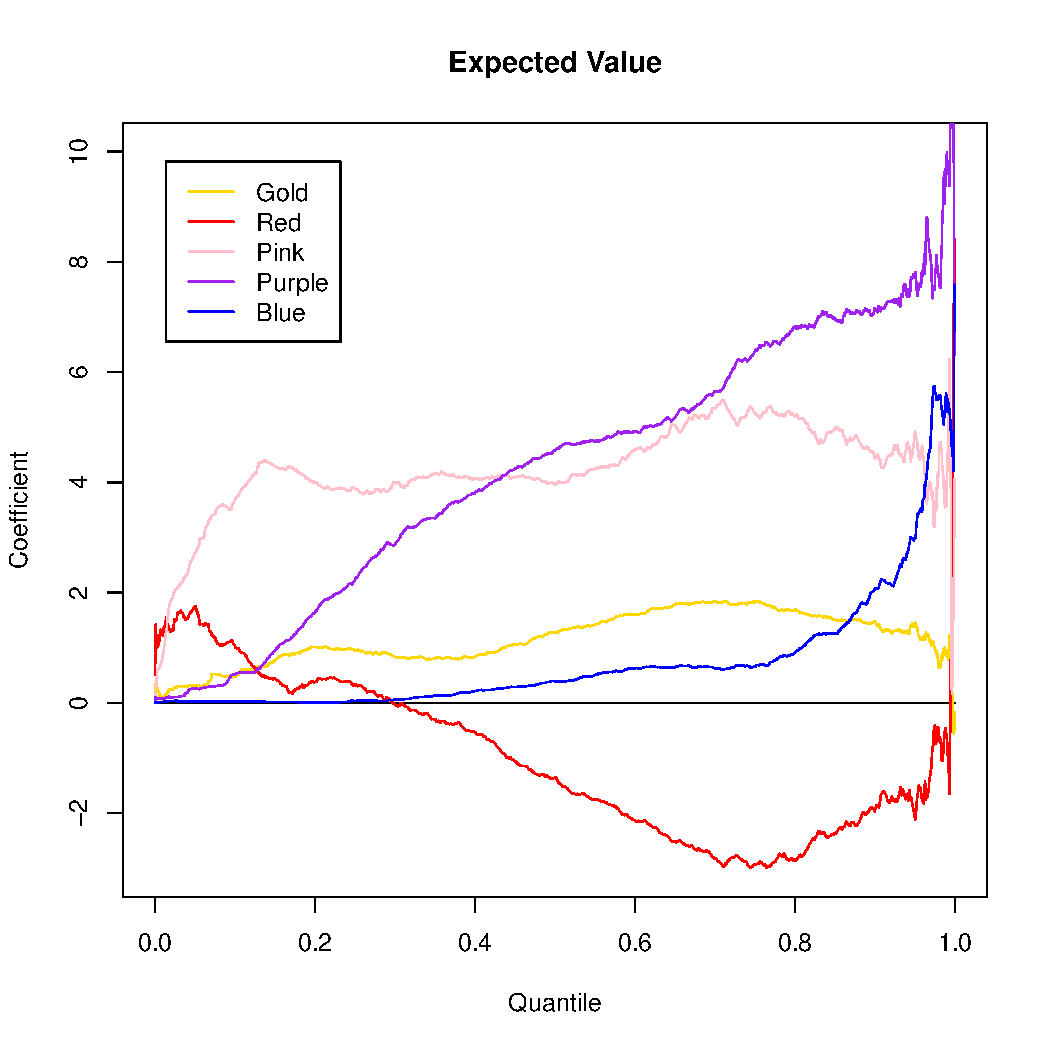
\includegraphics[width=.9\linewidth]{../Plots/QuantRegQuality.pdf}
\end{frame}

\begin{frame}[label=sec-1-41]{Loot box Averages}
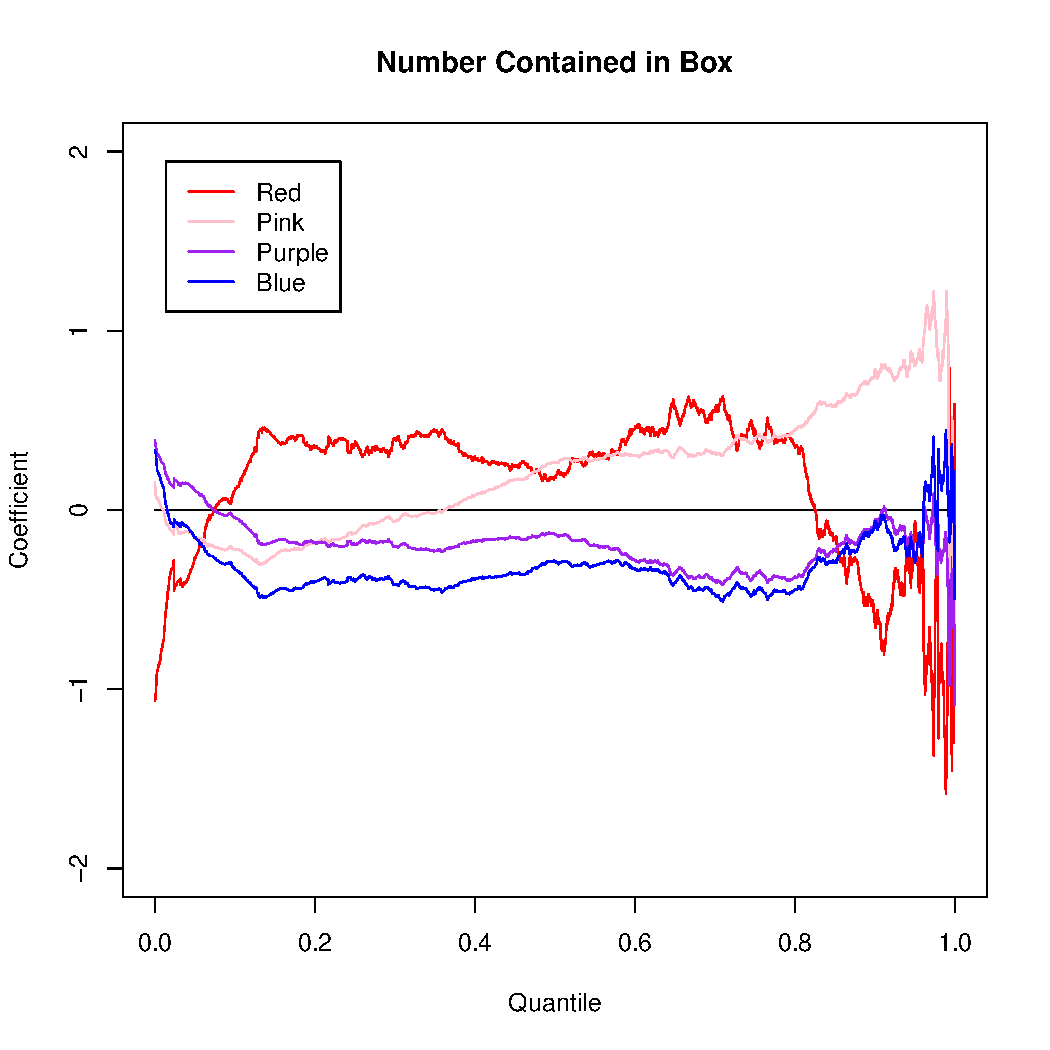
\includegraphics[width=.9\linewidth]{../Plots/QuantRegNumInBox.pdf}
\end{frame}

\begin{frame}[label=sec-1-42]{Loot box Averages}
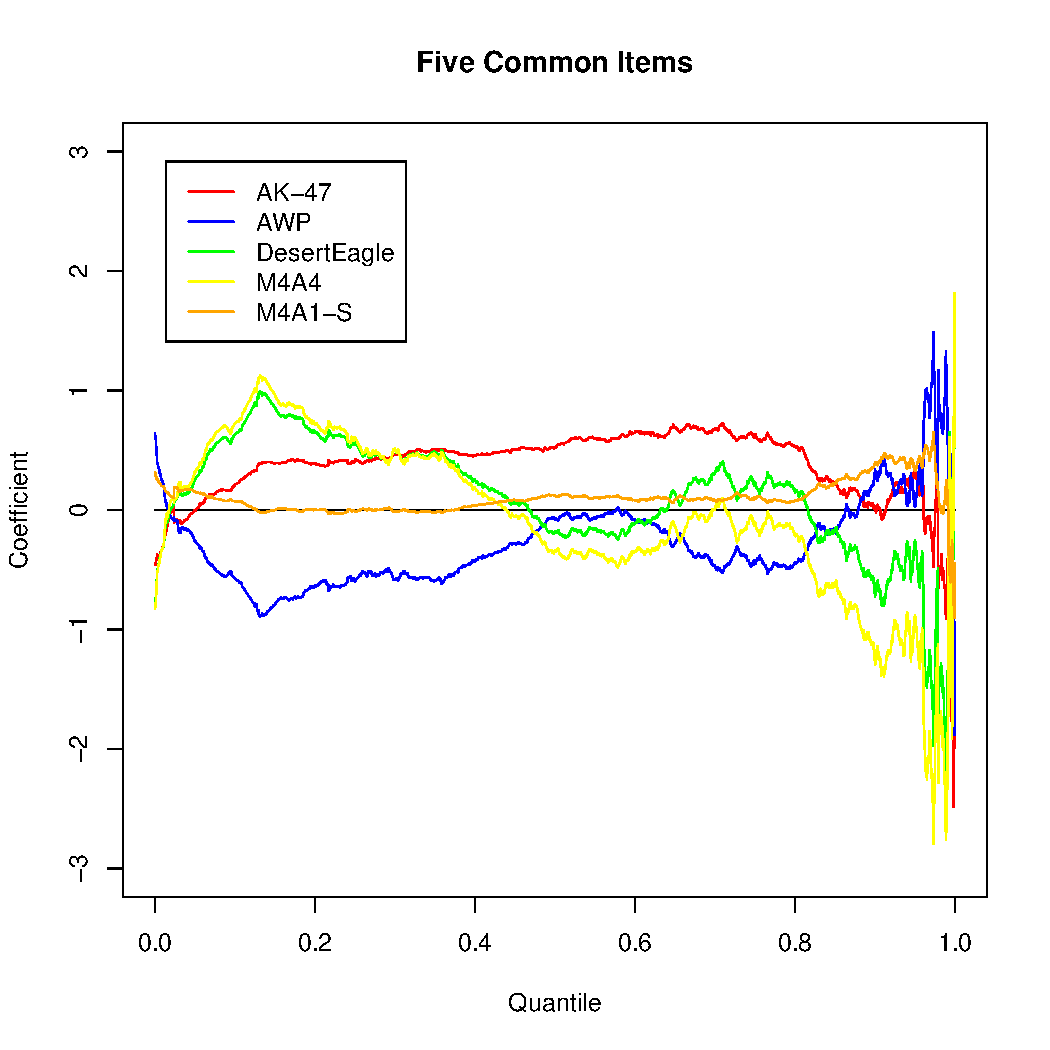
\includegraphics[width=.9\linewidth]{../Plots/QuantRegGuns.pdf}
\end{frame}
% Emacs 25.3.1 (Org mode 8.2.10)
\end{document}